\section{ Herleitung Selbstkonsistenzgleichung }

\begin{frame}
	\frametitle{ Das Modell }
    \begin{itemize}
        \item Tight-Binding Hüpfterm mit zusätzlichen Hubbard-Term
        \begin{align*}
            \oH = - \sum_{n,\mathbf{R}, \mathbf{R'}} t_n(\mb{R}-\mb{R'}) \ocd{n}(\mb{R}) \oc{n}(\mb{R'}) - U \sum_{\mb{R}} \op{n}^\dagg_{\mb{R}, \uparrow} \op{n}_{\mb{R}, \downarrow}
        \end{align*}
        \item $U>0$ und negatives Vorzeichen wegen Supraleitung
        \item Verwende Nearest-Neighbour Näherung und betrachte nur s-Band Elektronen
        \begin{align*}
            \oH = -t \sum_{\nearest{\mb{R}}{\mb{R'}}, \sigma} \ocd{\sigma}(\mb{R}) \oc{\sigma}(\mb{R'}) - U \sum_{\mb{R}} \op{n}^\dagg_{\mb{R}, \uparrow} \op{n}_{\mb{R}, \downarrow}
        \end{align*}
    \end{itemize}
\end{frame}

\begin{frame}
	\frametitle{ Bienenwabengitter }
    \begin{minipage}[t]{0.7\textwidth}
        \begin{itemize}
            \item 2 zueinander verschobene Dreiecksgitter mit Basispunkten $A$ und $B$.
            \item Gittervektoren sind 
            \begin{align*}
                \mb{a_1} &= \frac{a}{2} \begin{pmatrix} 3 \\ \sqrt{3} \end{pmatrix} & & \text{und} & \mb{a_2} &= \frac{a}{2} \begin{pmatrix*} 3 \\ -\sqrt{3}
                \end{pmatrix*}
            \end{align*}
            \item Nearest-Neighbour-Vektoren sind
            \begin{align*}
                \bdelta_1 &= \frac{a}{2} \begin{pmatrix} 1 \\ \sqrt{3} \end{pmatrix} & \bdelta_2 &= \frac{a}{2} \begin{pmatrix*} 1 \\ -\sqrt{3} \end{pmatrix*} & \bdelta_3 &= a \begin{pmatrix} -1 \\ 0 \end{pmatrix} 
            \end{align*}
            \item Führe fermionische Erzeuger-/Vernichter Operatoren $\oA_{\mb{R}}$ und $\oB_{\mb{R'}}$ ein
            \begin{equation*}
                \implies \oH = -t \sum_{\mb{R}, \bdelta, \sigma} \oad{\mb{R}} \ob{\mb{R} + \bdelta} + h.c. - U \sum_{\mb{R}} \sum_{\oC} \op{n}^\dagg_{\oC, \mb{R}, \uparrow} \op{n}_{\oC, \mb{R}, \downarrow}
            \end{equation*}
        \end{itemize}
    \end{minipage}
    \begin{minipage}[t]{0.29\textwidth}
        \vspace{-1cm}
        \begin{figure}
            \centering
            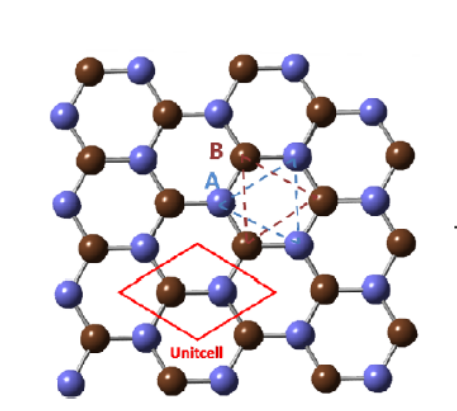
\includegraphics[width=\textwidth]{images/gitter.png}
        \end{figure}
    \end{minipage}
\end{frame}

\begin{frame}
	\frametitle{ Fouriertrafo }
    \begin{itemize}
        \item Nutze Tranlsationsinvarianz aus mit Fouriertrafo 
        \begin{align*}
            \oc{\mb{R}} &= \frac{1}{\sqrt{N}} \sum_{\mb{k}} \oa{\mb{k}} e^{\im \mb{k}\cdot \mb{R}} & \ocd{\mb{R}} &= \frac{1}{\sqrt{N}} \sum_{\mb{k}} \oa{\mb{k}} e^{- \im \mb{k}\cdot \mb{R}}
        \end{align*}
        \item Hüpfterm wird dann zu 
        \begin{align*}
            \oH_{\text{Hüpf}} &= \sum_{\mb{k}, \sigma} \underbrace{\sum_{\bdelta} -t e^{\im \mb{k}\cdot \bdelta}}_{:= f(\mb{k}) } \oad{\mb{k}, \sigma} \ob{\mb{k}, \sigma} + h.c. = \sum_{\mb{k}, \sigma} f(\mb{k}) \oad{\mb{k}, \sigma} \ob{\mb{k}, \sigma} + h.c.
        \end{align*}
        \item Hubbardterm nach ein paar mehr Umformungsschritten
        \begin{align*}
            \oH_{\text{Hubb}} &= -\frac{U}{N} \sum_{\oC} \sum_{\mb{k},\mb{k'},\mb{q}} \ocd{\mb{k}+\mb{q}, \uparrow} \ocd{\mb{k'} - \mb{q},\downarrow} \oc{\mb{k'}, \downarrow} \oc{\mb{k}, \uparrow}
        \end{align*}
    \end{itemize}
\end{frame}

\begin{frame}
	\frametitle{ Mean Field Näherung (1)}
    \begin{itemize}
        \item Wende Mean Field Näherung auf Hubbardterm an 
        \begin{align*}
            \ocdu \ocdd \ocndd \ocndu &\approx\ocdu \ocdd \underbrace{\expval{\ocndd \ocndu}}_{\propto \delta_{\mb{k}, -\mb{k'}}} + \expval{\ocdu \ocdd} \ocndd \ocndu \\
            &- \ocdu \ocndd \underbrace{\expval{\ocdd \ocndu}}_{= 0} - \expval{\ocdu \ocndd} \ocdd \ocndu \\
            &+ \ocdu \ocndu \underbrace{\expval{\ocdd \ocndd}}_{\propto \delta_{\mb{q}, \mb{0}}} + \expval{\ocdu \ocndu} \ocdd \ocndd + \text{const.}
        \end{align*}
        \item Damit ergibt sich der BCS-Term
        \begin{align*}
            \mathbf{T}_1 &= - \sum_{\mb{k}} \left(\Delta_{\oA} \oad{\mb{k},\uparrow} \oad{-\mb{k}, \downarrow} + \Delta_{\oB} \obd{\mb{k}, \uparrow} \obd{-\mb{k}, \downarrow}  \right) + h.c.
        \end{align*}
        mit Ordnungsparametern
        \begin{align*}
            \Delta_{\oC} &= \frac{U}{N} \sum_{\mb{k'}} \expval{\oc{-\mb{k'}, \downarrow } \oc{\mb{k'}, \uparrow} }
        \end{align*}
    \end{itemize}
\end{frame}

\begin{frame}
	\frametitle{ Mean Field Näherung (2) }
    \begin{itemize}
        \item Für den Hartree-Erwartungswert ergibt sich 
        \begin{align*}
            \mathbf{T}_2 &= - \sum_{\mb{k}, \sigma, \sigma'} (1 - \delta_{\sigma, \sigma'}) \left( \mu_{\oA, \sigma'} \oad{\mb{k}, \sigma} \oa{\mb{k}, \sigma} + \mu_{\oB, \sigma'} \obd{\mb{k},\sigma} \ob{\mb{k}, \sigma} \right)
        \end{align*}
        mit chemischen Potentialen 
        \begin{align*}
            \mu_{\oC, \sigma'} &= \frac{U}{N} \sum_{\mb{k'}} \expval{ \ocd{\mb{k'}, \sigma'} \oc{\mb{k'}, \sigma'} }
        \end{align*}
        \item Zur Vereinfachung nehme hier halbe Füllung an, also $\mu_{\oC, \sigma'} = 0$
        \item Damit ergibt sich der Hamiltonian 
        \begin{align*}
            \oH &= \sum_{\mb{k}, \sigma} f(\mb{k}) \oad{\mb{k}, \sigma} \ob{\mb{k},\sigma} - \sum_{\mb{k}} \left(\Delta_{\oA} \oad{\mb{k},\uparrow} \oad{-\mb{k}, \downarrow} + \Delta_{\oB} \obd{\mb{k}, \uparrow} \obd{-\mb{k}, \downarrow}  \right) + h.c.
        \end{align*}
    \end{itemize}
\end{frame}

\begin{frame}
	\frametitle{ Diagonalisiere Hamiltonian (1)}
    \begin{itemize}
        \item Verwende Nambu-Spinor $\vec{\Psi} = \left(\oad{\mb{k}, \uparrow} , \obd{\mb{k}, \uparrow} , \oa{-\mb{k}, \downarrow} , \ob{-\mb{k}, \downarrow}\right)^T$ 
        \begin{align*}
            \oH &= \sum_{\mb{k}} \Psi^\dagg \underline{\underline  {h}} \Psi  & &\text{mit} & \underline{\underline  {h}} &= \begin{pmatrix}
                0 & -f^* & \Delta_{\oA} & 0 \\
                -f & 0 & 0 & \Delta_{\oB} \\
                \Delta_{\oA} & 0 & 0 & f^* \\
                0 & \Delta_{\oB} & f & 0
            \end{pmatrix}
        \end{align*}
        \item  Zur weiteren Vereinfachung nehme hier an, dass $\Delta_{\oA} = \Delta_{\oB} \equiv \Delta$ gilt
        \item Gültigkeit dieser Annahme noch zu überprüfen
    \end{itemize}
\end{frame}

\begin{frame}
	\frametitle{ Diagonalisiere Hamiltonian (2)}
    \begin{itemize}
        \item diagonalisiere $\underline{\underline{h}}$ mit unitärer Trafo $U^\dagg$
        \begin{align*}
            U^\dagg &= \frac{1}{\sqrt{2}}\begin{pmatrix}
                1 & 0 & -1 & 0 \\
                -\frac{f}{E_\mb{k}} & \frac{\Delta}{E_\mb{k}} & -\frac{f}{E_\mb{k}} & -\frac{\Delta}{E_\mb{k}} \\
                \frac{\Delta}{E_\mb{k}} & -\frac{f^*}{E_\mb{k}}  & \frac{\Delta}{E_\mb{k}} & -\frac{f^*}{E_\mb{k}} \\
                0 & 1 & 0 & 1
            \end{pmatrix} 
            & \text{mit} & &E_\mb{k} &= \sqrt{\Delta^2 + \abs{f}^2}
        \end{align*}
        \begin{align*}
            \implies \oH &= \sum_\mb{k} E_\mb{k} \left( \ophioned \ophione + \ophitwod \ophitwo - \ophithreed \ophithree - \ophifourd \ophifour  \right) \\
            \intertext{und} \vec{\varphi} &= \left(\ophione, \ophitwo, \ophithree, \ophifour\right)^T = U^\dagg \vec{\Psi}
        \end{align*}
    \end{itemize}
\end{frame}

\begin{frame}
	\frametitle{ Selbstkonsistenz }
    \begin{itemize}
        \item Einsetzen von Inverser Trafo $\vec{\Psi} = U \vec{\varphi}$ in Definition von $\Delta$ 
        \begin{align*}
            \Delta &= \frac{U}{N} \sum_{\mb{k'}} \expval{\oa{-\mb{k'}, \downarrow } (\vec{\varphi}) \oa{\mb{k'}, \uparrow}(\vec{\varphi}) } \\
            &= \frac{U}{N} \sum_{\mb{k}} \frac{\Delta}{E_\mb{k}} \left( \expval{\ophione \ophioned } - \expval{\ophithree \ophithreed}\right) + \underbrace{\dots}_{=0} \\
            &= \frac{U}{N} \sum_{\mb{k}} \frac{\Delta}{E_\mb{k}} \tanh \left(\frac{\beta E_\mb{k}}{2}\right)
        \end{align*}
        \item Im Vergleich zu BCS-Theorie mit einem Band fehlt hier Faktor $2$ im Nenner
        \item Mit DOS und Cutoff durch Debye-Frequenz 
        \begin{align*}
            \Delta &= U \int_{-\hbar \omega_D}^{\hbar \omega_D} \rho(\epsilon) \frac{\Delta}{\sqrt{\Delta^2 + \epsilon^2}} \tanh\left(\frac{\beta \sqrt{\Delta^2 + \epsilon^2}}{2}\right) \, \diff \epsilon
        \end{align*}
    \end{itemize}
\end{frame}

\section{Numerische Lösung}

\begin{frame}
    \frametitle{Erste Ergebnisse}
        \begin{figure}
            \centering
            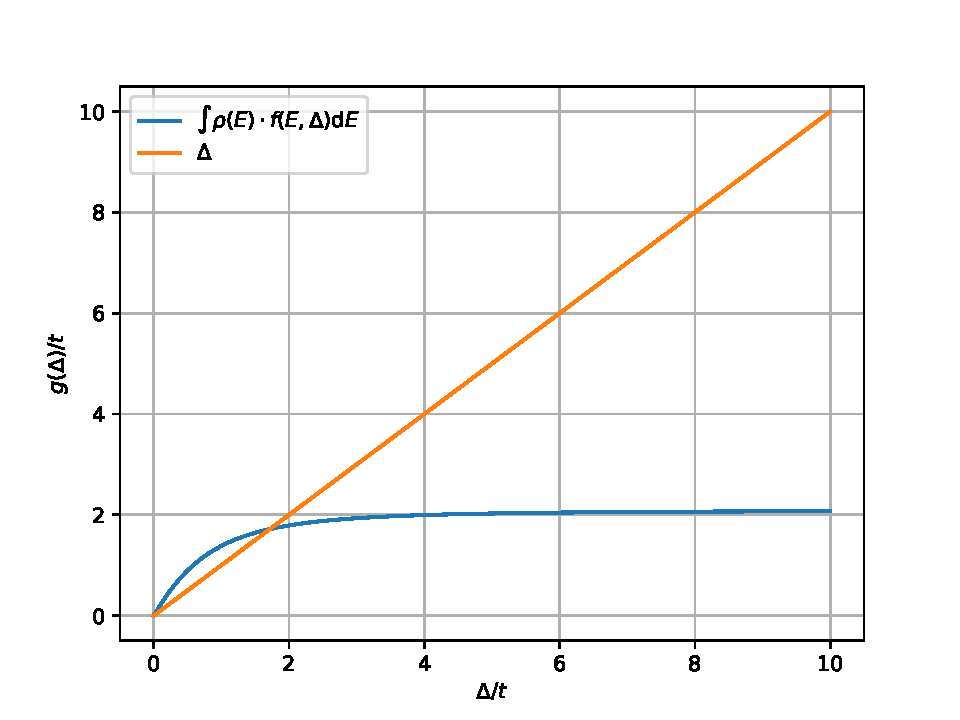
\includegraphics[width=0.6\textwidth]{images/schnittpunkte.pdf}
        \end{figure}
\end{frame}

\begin{frame}
    \frametitle{$\Delta$-Abhängigkeiten (1)}
    \begin{figure}
        \centering
        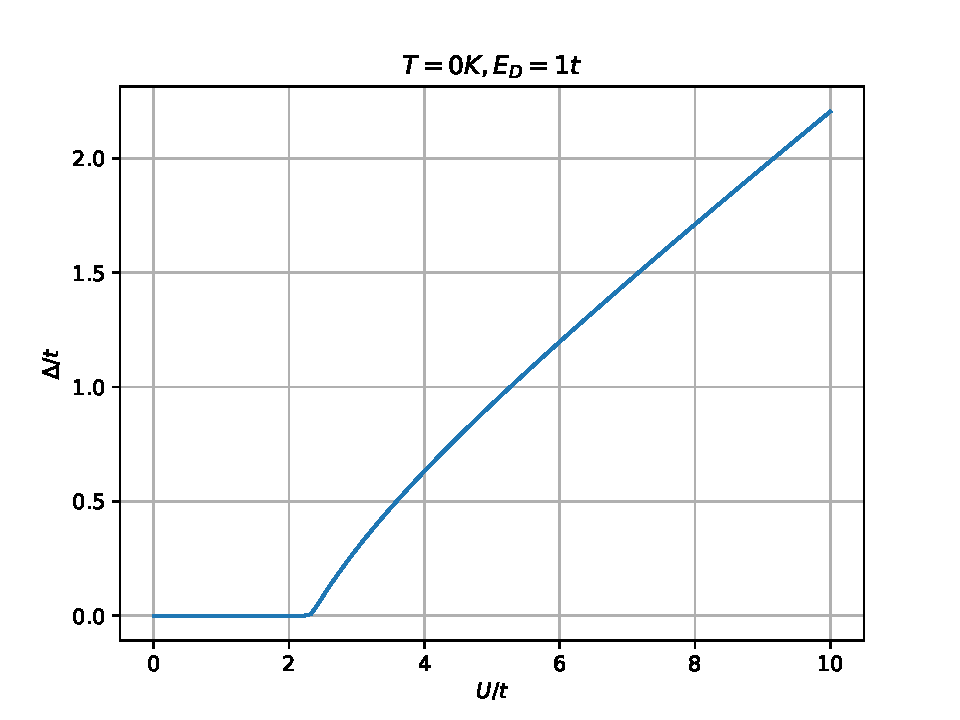
\includegraphics[width=0.6\textwidth]{images/U_vs_delta.pdf}
    \end{figure}
\end{frame}

\begin{frame}
    \frametitle{$\Delta$-Abhängigkeiten (2)}
    \begin{figure}
        \centering
        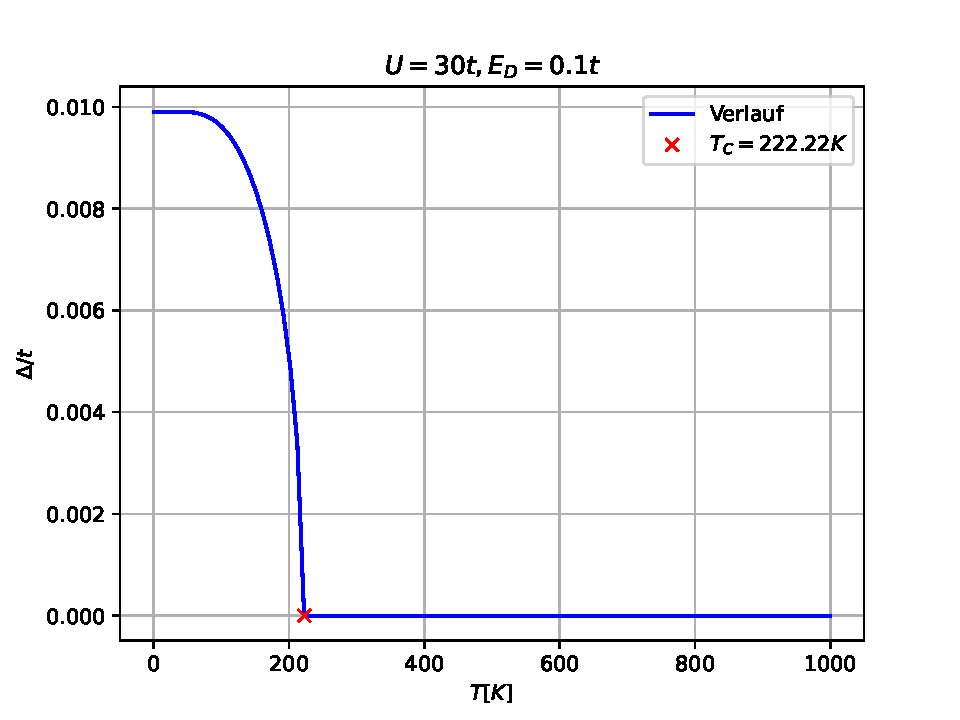
\includegraphics[width=0.6\textwidth]{images/T_vs_delta.pdf}
    \end{figure}
\end{frame}

\begin{frame}
    \frametitle{$\Delta$-Abhängigkeiten (3)}
    \begin{figure}
        \centering
        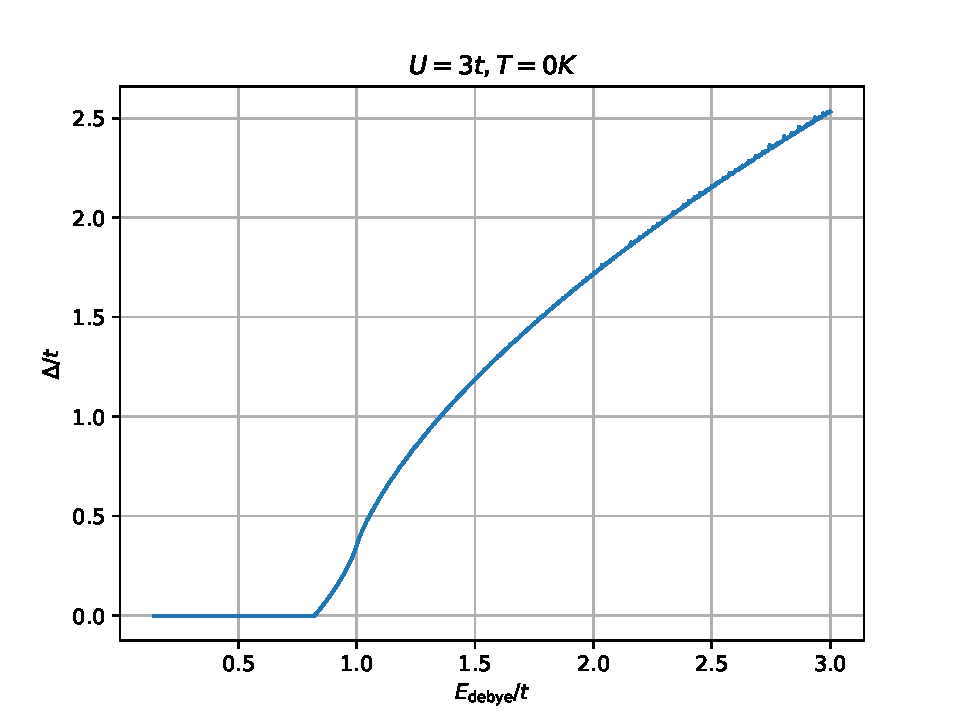
\includegraphics[width=0.6\textwidth]{images/Debye_vs_delta.pdf}
    \end{figure}
\end{frame}